%
%
%   KADONO
%
%

% 11/12 2:00 nakayama が編集しました。
% 11/14 13:45 nakayama が編集しました。


\documentclass[11pt,b5paper,papersize,dvipdfmx]{jsbook}

\usepackage{vuccaken}
\usepackage{vuccaken2018}
\usepackage{14kadono}


% 以下本文
\begin{document}
% \tableofcontents % 目次出力

% - - - - - - - - - - - - - - - - - - - - - - - - - - -
\kaishititle{Pythonでデータ処理}{物理科学科4回生}{門野広大}
% - - - - - - - - - - - - - - - - - - - - - - - - - - -

%
\section*{はじめに}
研究室に入ったら実験データをグラフにプロットしたりいろんなことをしないといけないと思います。研究室によってデータ処理をするソフトは異なると思いますが、大体は有料で個人で買うにはちょっと…っていう感じになると思います。研究室で作業すれば問題はないと思いますが、家でゆっくり一人で作業したいけど研究室のパソコンをもってかえるのはだるいといった感じになります。\par
そういうときにPythonで簡単なデータ処理ができるようになっているといいと思います。それならGnuplotでいいじゃんかという声がしそうなのでちょっと補足しておきます。Pythonはデータ処理だけでなくいろんなことができるのでデータ処理から入って数値解析などに進展したりすることも数値計算の知識さえあれば簡単にできます。それに今絶賛流行中のラズパイも基本的にPythonでプログラミングします。そのほかにもこれから出てくるマイコン(マイクロコンピュータ)の開発環境はPythonが増えると思います。データ分析から入ってPythonの世界に入れば研究の可能性が広がっていきます。\par
今回の会誌は、実験データをプロットして簡単なフィッティングできるまで解説したいと思います。(自分も初心者なので信用しきらないで下さい)
\section{環境構築}
%
\subsection{諸注意}
Pythonを書く環境は調べるとたくさんあり今回紹介するのはあくまで一例なのでまあ気に入らなかったら別の環境にすぐさま移動してください。
%
\subsection{vscode}
Visual Studio Code (vscode)でのPython構築をします。とっても簡単です。\par
まずvscodeをダウンロードします。\url{https://code.visualstudio.com/}からインストーラーをダウンロードして、起動させてください。追加タスクの選択をすべて選択しておくと今後便利かも。\par
次に、vscodeの拡張機能を追加します。ファイル→基本設定→拡張機能でPythonで検索して一番上にあるやつをインストールしてください。インストールが完了したら再読み込みして、新規ファイルを作成し、
\begin{kdncode-i}
    print ('Hello world')
\end{kdncode-i}
と書き込み、拡張子を\tkdncode{.py}のファイル名で保存すると右下にPythonがダウンロードされてません的な警告が出るので、ダウンロードボタンを押してください。そうするとブラウザが開くのでそのサイトからインストーラーをダウンロードして起動してください。インストーラーの最初の画面にpathの追加云々のチェックがあるのでチェックしてください。そこから先は特に特別なことをしなくても大丈夫です。ダウンロードが終わったら、再度vscodeを開き先ほど保存したファイルを開いてください。\par
F5をクリックするだけでデバックができるのでクリックしてください。そうすると下のほうにターミナルが開くので、そのになんか黄色い文字が表示され、なんかコマンドを実行してくださいできなことが書いてあったらそのコマンドをターミナルに書き込んで実行してください。おそらく
\begin{kdncode-ii}
    python -m pip install -U pylint --user
    python -m pip install --upgrade pip
\end{kdncode-ii}
の二つだと思います。\par
以上でおそらく環境が構築できると思いますが何か行き詰まったらGoogle先生に聞いてください。いろんな人が詳しくブログで紹介してくれているのでこんな適当な説明よりも百倍いいと思います。

%
\subsection{ライブラリの追加方法}
この後、初期状態では入っていないライブラリを使用します。コマンド一つで追加することができます。デバックを開始したときに入ってないぞと言われたら\tkdncode{import}や\tkdncode{from}とかの後ろに書いてあるライブラリの名前を以下のコマンドに入れてターミナルで実行してください。
\begin{kdncode-ii}
    import numpy as np
\end{kdncode-ii}
↑これだったらライブラリの名前=\tkdncode{numpy}
\begin{kdncode-ii}
    from matplotlib import pyplot
\end{kdncode-ii}
↑これだったらライブラリの名前=\tkdncode{matplotlib} \par
コマンド
\begin{kdncode-ii}
    python -m pip install ライブラリの名前
\end{kdncode-ii}

%
\section{Pythonの基礎}
今回使用する主な文法についてだけです。詳しくは本やブログを参照してください。

%
\subsection{主な形}
Pythonのプログラム(Pythonには限らず)は基本的に上から順番に実行していきます。初めにライブラリを追加するプログラムを入れます。
\begin{kdncode-ii}
    from matplotlib import pyplot
    import numpy as np
    import math
\end{kdncode-ii}
\begin{kdncode-i}
    import + ライブラリの名前
\end{kdncode-i}
で基本的にできます。ライブラリでそのプログラムで用意されている関数をしようするとき
\begin{kdncode-i}
    ライブラリの名前.関数名()
\end{kdncode-i}
のような形で使用しないといけないので、ライブラリの名前が長いと面倒なので
\begin{kdncode-i}
    import + ライブラリの名前 + as + 今後使用する名前
\end{kdncode-i}
といった形に書いてやると関数の名前を短くできます。\par
ライブラリを追加したらそのあとは普通にプログラムを書くだけです。\par
自作の関数を作成するには
\begin{kdncode-ii}
    def func(x ,intensity ,X0,HWHM):
        return intensity * HWHM**2 /((x-X0)**2 + HWHM**2)
\end{kdncode-ii}
といった形で書けます。上はローレンツ関数の値を返す関数です。

%
\subsection{条件分岐}
\begin{kdncode-ii}
    if 条件1:
        処理1
    elif 条件2:
        処理2
    else:
        処理3    
\end{kdncode-ii}
という形です。

%
\subsection{繰り返し}
この処理がPythonでは遅いらしいです。あんま使わないで用意されている関数をうまく使用してください。\par
C言語とはちょっと違います。C言語とかはカウンタ変数(大体$i,j$とか使うやつ)をどこまでやるかみたいな感じでループをしますが、Pythonではそういうものは使わないっぽいです。下に具体例を示します。
\begin{kdncode-ii}
    l = ['Alice', 'Bob', 'Charlie']
    for name in l:
        print(name)
\end{kdncode-ii}
\tkdncode{for}の後に任意の適当な変数を入れループは\tkdncode{in}の後のリストなどのインテラブルオブジェクト?の要素が順番に変数が代入され処理が行われるっぽいです。\par
通常のC言語みたいなループをしたい場合は\tkdncode{range()}関数を使用します。\par
\tkdncode{range(最小値,最大値,数)}のように引数をとると最小値から最大値まで指定した数だけのリストを作ってくれます。普通に何回か同じ処理を繰り返したいだけだったら、\tkdncode{range(回数)}という形で引数をとればその回数だけループを繰り返してくれます。回数は任意の変数に代入されます。\par
下に\tkdncode{range()}を使った例を示します。
\begin{kdncode-ii}
    for name in range(100):
        sum = sum + 1
\end{kdncode-ii}
\par\par
ほかにもたくさんありますが、詳しくは書店にあるPythonの本を読んでください。とても丁寧に書いてあります。
\section{データの処理}
とりあえず今回は自分が実験に使用したプログラムについての解説的な感じにしたいと思います。すべて理解している人が書いているわけではないのでその辺察してくれるとありがたいです。
\subsection{データ処理のプログラム全体図}
とりあえず自分が実験データのフィッティングに使用したものを下にコピペします。ほとんど誰かのブログのパクリです。
\begin{kdncode-ii}
    import numpy as np
    from matplotlib import pyplot
    import matplotlib.ticker as ptick
    import scipy.optimize
    import glob, re
    from functools import cmp_to_key

    filename = 'file.dat'

    with open(filename,'r') as file:
        X,Y =[],[]
        for line in file.readlines()[0:]:
            items = line[:-1].split(' ')
            X.append(float(items[0]))
            Y.append(float(items[1]))
    pyplot.plot(X,Y,label = filename)

    max_Y = max(Y)
    min_Y = min(Y)

    if np.abs(max_Y) >= np.abs(min_Y):
        intensity = max_Y 
        X0 = X[Y.index(max_Y)]
    else:
        intensity = min_Y
        X0 = X[Y.index(min_Y)]

    pini = np.array([intensity,X0,1])

    def func(x ,intensity ,X0,HWHM):
        return intensity * HWHM**2 /((x-X0)**2 + HWHM**2)

    popt, pcov = scipy.optimize.curve_fit(func, X, Y, p0=pini)
    perr = np.sqrt(np.diag(pcov))

    print("initial parameter\toptimized parameter")
    for i, v  in enumerate(pini):
            print(str(v)+ '\t' + str(popt[i]) + ' ± ' + str(perr[i]))

    fitline = func(X, popt[0], popt[1], popt[2])
    pyplot.plot(X, fitline,label = 'FITTING')
    pyplot.ylabel('intensity',fontsize = 15)
    pyplot.xlabel('Shift[GHz]',fontsize = 15) 
    pyplot.tick_params(labelsize = 12)
    pyplot.legend(loc="best")  
    pyplot.show()
\end{kdncode-ii}
このプログラムはデータファイルを読み込んで、ローレンチアンでフィッティングしようというものです。ローレンチアンって何かというと、
式で書くと
\begin{align*}
    f(x) = I_0\frac{(\Gamma/2)^2}{(x - x_0)^2 + (\Gamma/2)^2}
\end{align*}
この式をグラフ化すると
\begin{figure}[H]
    \centering
    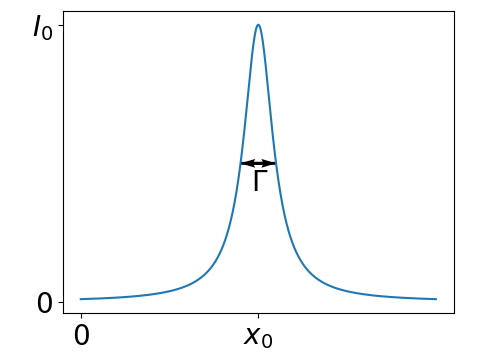
\includegraphics[height=32mm]{kadono/img/rorent.png}
    \caption{ローレンチアン}
    \label{fig:rorent}
\end{figure}\vspace{-1zw}
この形の関数は割とよくある形です。このフィッティングができたら大体良いです。
上のプログラムの各部分をちょっと詳しく…
\subsection{データプロット}
はじめにデータ処理をするうえでデータを読み込ませないといけないです。上のプログラムでは初めに行っています。
\begin{kdncode-ii}
    filename = 'file.dat'
    
    with open(filename,'r') as file:
        X,Y =[],[]
        for line in file.readlines()[0:]:
            items = line[:-1].split(' ')
            X.append(float(items[0]))
            Y.append(float(items[1]))
    pyplot.plot(X,Y,label = filename)
\end{kdncode-ii}
この部分です。\tkdncode{filename}には今から処理したいデータのファイル名を入れてください。拡張子は \tkdncode{*.txt,*.dat,*.plt} はできました。他は知りませんが多分大丈夫です。
\begin{kdncode-i}
    with open(filename,'r') as file:
\end{kdncode-i}
この後にファイルを読み込む動作を書きます。通常だとファイルを開いて処理してファイルを閉じるといった操作をしなくてはならないですが、これはしなくてよさそうです。
\begin{kdncode-i}
    X,Y =[],[]
\end{kdncode-i}
では、これからファイルから読み込むデータの配列を宣言してます。
\begin{kdncode-i}
    for line in file.readlines()[0:]:
\end{kdncode-i}
で、のループで最後まで読み込んでます。\tkdncode{file.readlines()[0:]}で何行目から読んでどこまで読まないかを宣言できます。ここでは一行目からファイルの最後までって感じです。
\begin{kdncode-i}
    item = line[:-1].split(' ')
\end{kdncode-i}
ここでデータファイルのデータが何で区切られてるのかを宣言します。\tkdncode{split('')}の中に入れます。上ではスペースですと書いてあります。タブの場合\verb|('\t')|、セミコロンの場合\tkdncode{(',')}です。ほかの場合は調べてください。大体デバック開始したらvscodeが教えてくれますが…\par
そのあとは配列に順序良く入れるという関数です。ここで、どんな変数なのかをちゃんと言わないと今後そのデータを処理できません。\par
そのままグラフにプロットさせたかったら、\tkdncode{matplotlib}のライブラリにある\tkdncode{pyplot}を使って
\begin{kdncode-i}
    pyplot.plot(x軸のデータ,y軸のデータ)
\end{kdncode-i}
でプロットできます。表示したかったら
\begin{kdncode-i}
    pyplot.show()
\end{kdncode-i}
と打ち込めばその時点でplotしたデータのグラフを表示してくれます。

%
\subsection{データのフィッティング}
フィッティングする関数は下の部分です。
\begin{kdncode-ii}
    pini = np.array([intensity,X0,1])

    def func(x ,intensity ,X0,HWHM):
        return intensity * HWHM**2 /((x-X0)**2 + HWHM**2)

    popt, pcov = scipy.optimize.curve_fit(func, X, Y, p0=pini)
    perr = np.sqrt(np.diag(pcov))
\end{kdncode-ii}
いざフィッティングする部分は
\begin{kdncode-i}
    popt, pcov = scipy.optimize.curve_fit(func, X, Y, p0=pini)
\end{kdncode-i}
の関数です。よくわかってなくそのまま使っているのでわからないのですが。引数に、フィッティングしたいグラフの関数、$x$軸データ、$y$軸データ、初期値を入れたらフィッティングしてくれます。データの読み込みとこのフィッティングまでの間の部分は適当な初期値を決めるところです。何となく読んで察してください。\par
\tkdncode{popt}に収束したパラメータ、\tkdncode{perr}に標準誤差が格納されます。\par
そのあとはグラフにプロットするためのものです。調べてください。

%
\section{最後に}
今回は自分がブログを見ながら生データにフィッティングするためのプログラムを作ったのでそれについての解説をしたいがために書いたものです。本当に参考程度で温かい目で見てほしいです。

% 参考文献
\sanko
\begin{enumerate}
\item \url{https://qiita.com/yokot2/items/f8920f65b1037ec7009d}
\end{enumerate}

\end{document}
%
% ファイトだよ!
% お疲れ様です!!!
%